\usetikzlibrary{arrows.meta,calc}
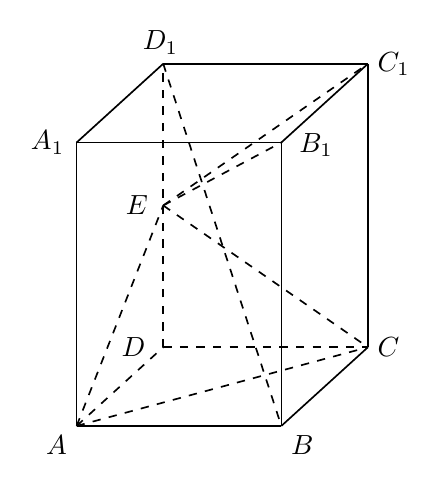
\begin{tikzpicture}[x=1cm,y=1cm,line width=.6pt,font=\normalsize]
\tikzset{ptlabel/.style={font=\normalsize,fill=white,inner sep=1.2pt}}
\coordinate (A) at (0,0);
\coordinate (B) at (2.6,0);
\coordinate (C) at (3.7,1.0);
\coordinate (D) at (1.1,1.0);
\coordinate (A1) at (0,3.6);
\coordinate (B1) at (2.6,3.6);
\coordinate (C1) at (3.7,4.6);
\coordinate (D1) at (1.1,4.6);
\coordinate (E) at (1.1,2.8);
\draw (A) -- (B);
\draw (B) -- (C);
\draw (B) -- (B1);
\draw (C) -- (C1);
\draw (A) -- (A1);
\draw (A1) -- (B1);
\draw (B1) -- (C1);
\draw (C1) -- (D1);
\draw (D1) -- (A1);
\draw[dashed] (A) -- (D);
\draw[dashed] (D) -- (C);
\draw[dashed] (A) -- (C);
\draw[dashed] (D) -- (D1);
\draw[dashed] (A) -- (E);
\draw[dashed] (E) -- (C);

\draw[dashed] (E) -- (B1);
\draw[dashed] (E) -- (C1);

\draw[dashed] (D1) -- (B);

\node[ptlabel,below left,xshift=-2pt,yshift=-2pt] at (A) {$A$};
\node[ptlabel,below right,xshift=2pt,yshift=-2pt] at (B) {$B$};
\node[ptlabel,right,xshift=2pt] at (C) {$C$};
\node[ptlabel,left,xshift=-3pt,xshift=-2.00bp,yshift=0.00bp] at (D) {$D$};
\node[ptlabel,left,xshift=-3pt] at (A1) {$A_{1}$};
\node[ptlabel,right,xshift=3pt,yshift=1pt,xshift=2.00bp,yshift=-2.00bp,fill=none] at (B1) {$B_{1}$};
\node[ptlabel,right,xshift=2pt] at (C1) {$C_{1}$};
\node[ptlabel,above,xshift=-1pt,yshift=2pt] at (D1) {$D_{1}$};
\node[ptlabel,left,xshift=-4pt] at (E) {$E$};
\end{tikzpicture}
